%% This is the ctufit-thesis example file. It is used to produce theses
%% for submission to Czech Technical University, Faculty of Information Technology.
%%
%% This is version 1.4.3, built 1. 4. 2025.
%% 
%% Get the newest version from
%% https://gitlab.fit.cvut.cz/theses-templates/FITthesis-LaTeX
%%
%%
%% Copyright 2024, Tomas Novacek
%% Copyright 2021, Eliska Sestakova and Ondrej Guth
%%
%% This work may be distributed and/or modified under the
%% conditions of the LaTeX Project Public License, either version 1.3
%% of this license or (at your option) any later version.
%% The latest version of this license is in
%%  https://www.latex-project.org/lppl.txt
%% and version 1.3 or later is part of all distributions of LaTeX
%% version 2005/12/01 or later.
%%
%% This work has the LPPL maintenance status `maintained'.
%%
%% The current maintainer of this work is Tomas Novacek (novacto3@fit.cvut.cz).
%% Alternatively, submit bug reports to the tracker at
%% https://gitlab.fit.cvut.cz/theses-templates/FITthesis-LaTeX/issues
%%
%%

% arara: xelatex
% arara: biber
% arara: xelatex
% arara: xelatex

%%%%%%%%%%%%%%%%%%%%%%%%%%%%%%%%%%%%%%%%%
% CLASS OPTIONS
% language: czech/english/slovak
% thesis type: bachelor/master/dissertation
% colour: bw for black&white OR no option for default colour scheme
% electronic (oneside) or printed (twoside), twoside is default
% paragraph - if passed, this optional argument sets paragraphs as the deepest level of headers, styles it, numbers it and adds it to Table of Content. Use with care! Normally, it is considered unwise to use it, since its too deep.
%%%%%%%%%%%%%%%%%%%%%%%%%%%%%%%%%%%%%%%%%
\documentclass[english,bachelor,oneside]{ctufit-thesis}

%%%%%%%%%%%%%%%%%%%%%%%%%%%%%%%%%%
% FILL IN THIS INFORMATION
%%%%%%%%%%%%%%%%%%%%%%%%%%%%%%%%%%
\ctufittitle{Grafit.games - Commercialization of Student Game Projects} % replace with the title of your thesis
\ctufitauthorfull{Samuel Černák} % replace with your full name (first name(s) and then family name(s) / surname(s)) including academic degrees
\ctufitauthorsurnames{Černák} % replace with your surname(s) / family name(s)
\ctufitauthorgivennames{Samuel} % replace with your first name(s) / given name(s)
\ctufitsupervisor{Bc. Ondřej Brém\, MSc.} % replace with name of your supervisor/advisor (include academic degrees)
\ctufitdepartment{Department of Software Engineering} % replace with the department of your defence
\ctufityear{2025} % replace with the year of your defence
\ctufitdeclarationplace{Praze} % replace with the place where you sign the declaration
\ctufitdeclarationdate{\today} % replace with the date of signature of the declaration
\ctufitabstractCZE{Fill in the abstract of this thesis in Czech. Lorem ipsum dolor sit amet. Class aptent taciti sociosqu ad litora torquent per conubia nostra, per inceptos hymenaeos. Cras pede libero, dapibus nec, pretium sit amet, tempor quis. Sed vel lectus. Donec odio tempus molestie, porttitor ut, iaculis quis, sem. Suspendisse sagittis ultrices augue.}
\ctufitabstractENG{Fill in the abstract of this thesis in English. Lorem ipsum dolor sit amet. Class aptent taciti sociosqu ad litora torquent per conubia nostra, per inceptos hymenaeos. Cras pede libero, dapibus nec, pretium sit amet, tempor quis. Sed vel lectus. Donec odio tempus molestie, porttitor ut, iaculis quis, sem. Suspendisse sagittis ultrices augue.}
\ctufitkeywordsCZE{enter, comma, separated, list, of, keywords, in, CZECH}
\ctufitkeywordsENG{enter, comma, separated, list, of, keywords, in, ENGLISH}
%%%%%%%%%%%%%%%%%%%%%%%%%%%%%%%%%%
% END FILL IN
%%%%%%%%%%%%%%%%%%%%%%%%%%%%%%%%%%

%%%%%%%%%%%%%%%%%%%%%%%%%%%%%%%%%%
% CUSTOMIZATION of this template
% Skip this part or alter it if you know what you are doing.
%%%%%%%%%%%%%%%%%%%%%%%%%%%%%%%%%%

\RequirePackage{iftex}[2020/03/06]
\iftutex % XeLaTeX and LuaLaTeX
    \RequirePackage{ellipsis}[2020/05/22] %ellipsis workaround for XeLaTeX
\else
    \errmessage{Only compilation with XeLaTeX or LuaLaTeX is allowed}
    \stop
\fi

% hyperlinks
\hypersetup{
    pdfpagelayout=TwoPageRight,
    colorlinks=false,
    allcolors=decoration,
    pdfborder={0 0 0.1}
}

% uncomment the following to hide all hyperlinks
%\hypersetup{hidelinks}

% uncomment the following to change the colour of all hyperlinks to CTU blue
%\hypersetup{allbordercolors=decoration}

\RequirePackage{pdfpages}[2020/01/28]

%%%%%%%%%%%%%%%%%%%%%%%%%%%%%%%%%%
% CUSTOMIZATION of this template END
%%%%%%%%%%%%%%%%%%%%%%%%%%%%%%%%%%


%%%%%%%%%%%%%%%%%%%%%%
% PACKAGES SETTINGS
% You may choose to modify this part.
%%%%%%%%%%%%%%%%%%%%%%
\usepackage{dirtree}
\usepackage{lipsum,tikz}
\usepackage[style=iso-numeric]{biblatex}
\addbibresource{text/bib-database.bib}
\usepackage{xurl}
\usepackage{listings} % typesetting of sources
%\usepackage{minted}
\usepackage{csquotes}

%%%%%%%%%%%%%%%%%%%%%%
% PACKAGES SETTINGS END
%%%%%%%%%%%%%%%%%%%%%%

\begin{document} 
\frontmatter\frontmatterinit % do not remove these two commands

\thispagestyle{empty}\maketitle\thispagestyle{empty}\cleardoublepage % do not remove these four commands

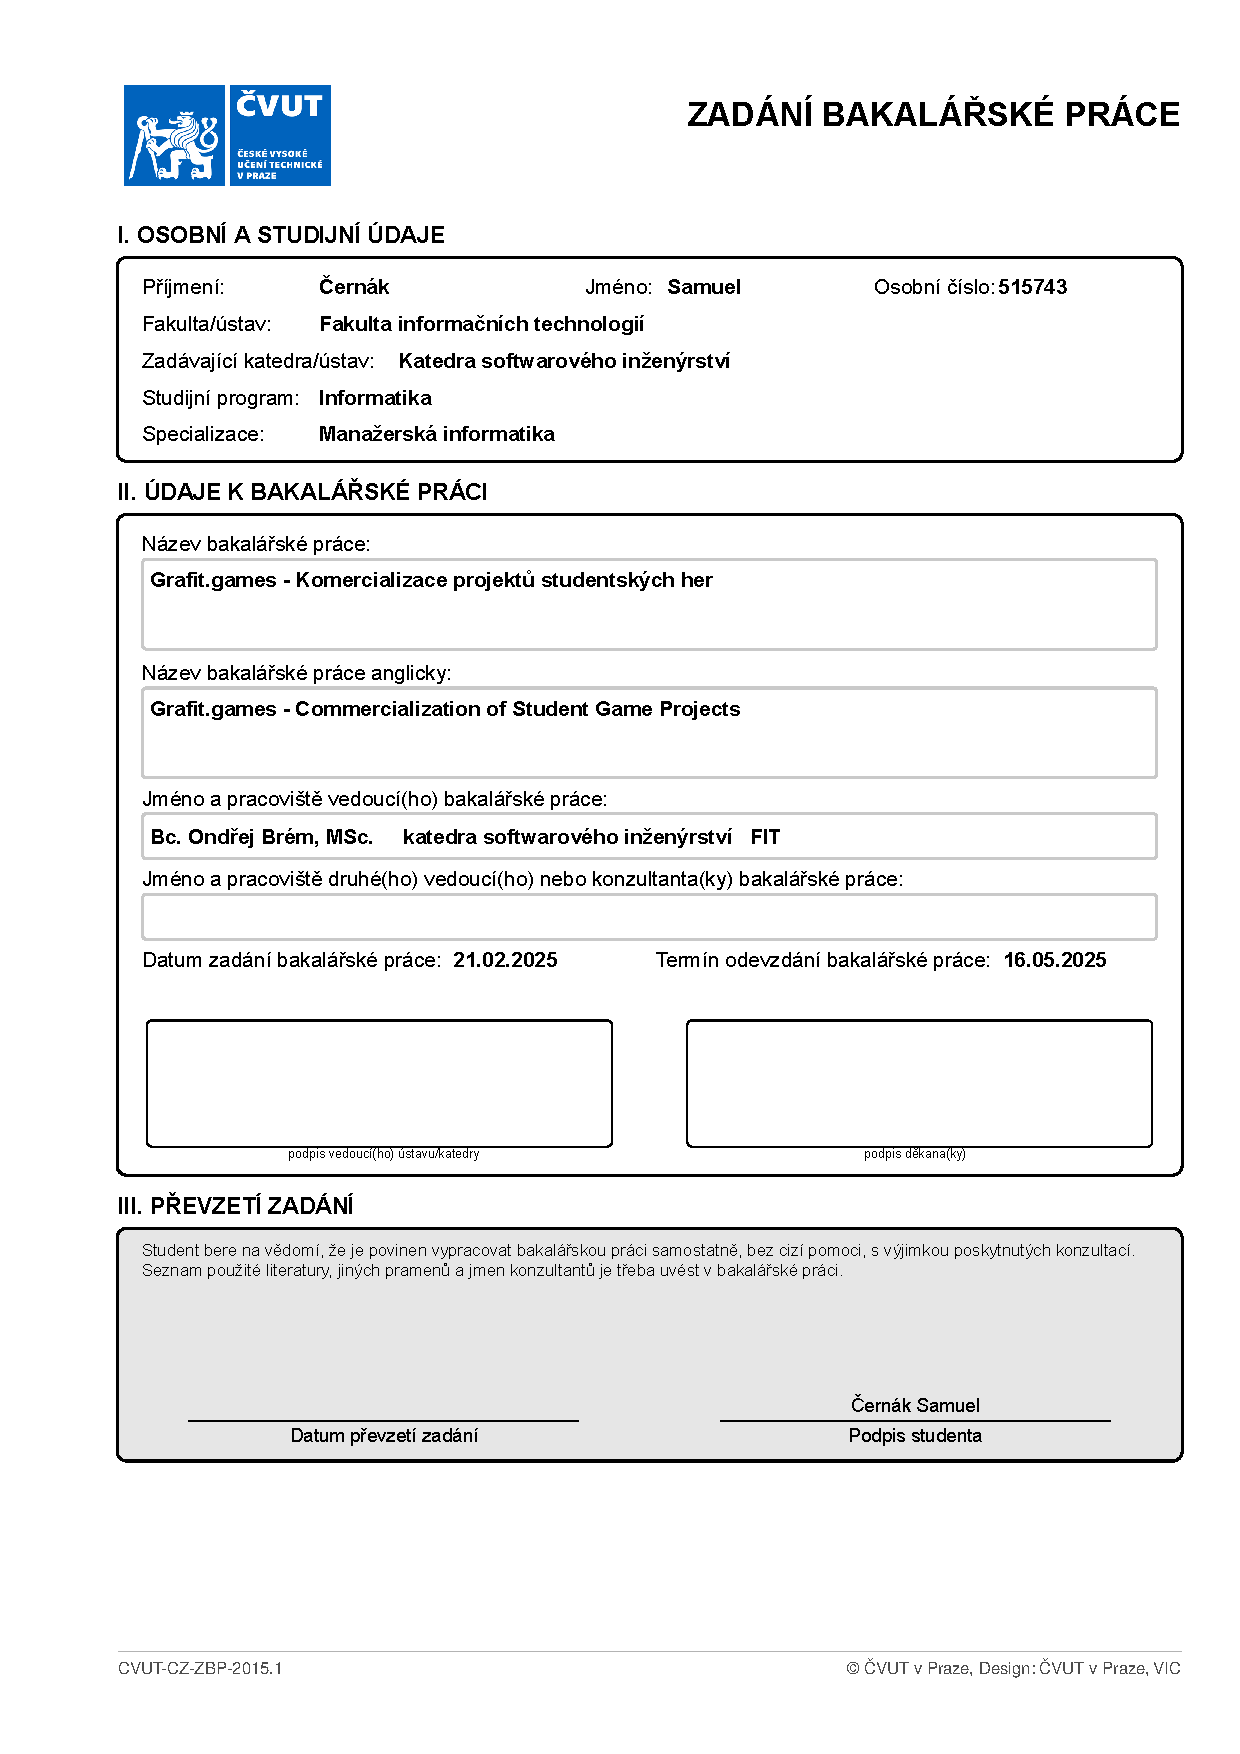
\includepdf[pages={1-}]{thesis-assignment.pdf} % replace this file with your thesis assignment generated from ProjectsFIT

\imprintpage % do not remove this command
\stopTOCentries
%%%%%%%%%%%%%%%%%%%%%%
% list of other contents END
%%%%%%%%%%%%%%%%%%%%%%

%%%%%%%%%%%%%%%%%%%
% ACKNOWLEDGMENT
% FILL IN / MODIFY
% This is a place to thank people for helping you. It is common to thank your supervisor.
%%%%%%%%%%%%%%%%%%%
\begin{acknowledgmentpage}
	Chtěl bych poděkovat především sit amet, consectetuer adipiscing elit. Curabitur sagittis hendrerit ante. Class aptent taciti sociosqu ad litora torquent per conubia nostra, per inceptos hymenaeos. Cras pede libero, dapibus nec, pretium sit amet, tempor quis. Sed vel lectus. Donec odio tempus molestie, porttitor ut, iaculis quis, sem. Suspendisse sagittis ultrices augue.
\end{acknowledgmentpage} 
%%%%%%%%%%%%%%%%%%%
% ACKNOWLEDGMENT END
%%%%%%%%%%%%%%%%%%%


%%%%%%%%%%%%%%%%%%%
% DECLARATION
% FILL IN / MODIFY
%%%%%%%%%%%%%%%%%%%
% INSTRUCTIONS
% ENG: choose one of approved texts of the declaration. DO NOT CREATE YOUR OWN. Find the approved texts at https://courses.fit.cvut.cz/SFE/download/index.html#_documents (document Declaration for FT in English)
% CZE/SLO: Vyberte jedno z fakultou schvalenych prohlaseni. NEVKLADEJTE VLASTNI TEXT. Schvalena prohlaseni najdete zde: https://courses.fit.cvut.cz/SZZ/dokumenty/index.html#_dokumenty (prohlášení do ZP)
\begin{declarationpage}
FILL IN ACCORDING TO THE INSTRUCTIONS. VYPLŇTE V SOULADU S POKYNY. Lorem ipsum dolor sit amet, consectetuer adipiscing elit. Curabitur sagittis hendrerit ante. Class aptent taciti sociosqu ad litora torquent per conubia nostra, per inceptos hymenaeos. Cras pede libero, dapibus nec, pretium sit amet, tempor quis. Sed vel lectus. Donec odio tempus molestie, porttitor ut, iaculis quis, sem. Suspendisse sagittis ultrices augue. Donec ipsum massa, ullamcorper in, auctor et, scelerisque sed, est. In sem justo, commodo ut, suscipit at, pharetra vitae, orci. Pellentesque pretium lectus id turpis.

Lorem ipsum dolor sit amet, consectetuer adipiscing elit. Curabitur sagittis hendrerit ante. Class aptent taciti sociosqu ad litora torquent per conubia nostra, per inceptos hymenaeos. Cras pede libero, dapibus nec, pretium sit amet, tempor quis. Sed vel lectus. Donec odio tempus molestie, porttitor ut, iaculis quis, sem. Suspendisse sagittis ultrices augue. Donec ipsum massa, ullamcorper in, auctor et, scelerisque sed, est. In sem justo, commodo ut, suscipit at, pharetra vitae, orci. Pellentesque pretium lectus id turpis.
\end{declarationpage}
%%%%%%%%%%%%%%%%%%%
% DECLARATION END
%%%%%%%%%%%%%%%%%%%

\printabstractpage % do not remove this command

%%%%%%%%%%%%%%%%%%%
% SUMMARY
% FILL IN / MODIFY
% OR REMOVE ENTIRELY (upon agreement with your supervisor)
% (appropriate to remove in most theses)
%%%%%%%%%%%%%%%%%%%
% \begin{summarypage}
% \section*{Summary section}
% 
% \lipsum[1][1-8]
% 
% \section*{Summary section}
% 
% \lipsum[2][1-6]
% 
% \section*{Summary section}
% 
% \lipsum[3]
% 
% \section*{Summary section}
% 
% \lipsum[2]
% 
% \section*{Summary section}
% 
% \lipsum[1][1-8] Lorem lorem lorem.
% \end{summarypage}
%%%%%%%%%%%%%%%%%%%
% SUMMARY END
%%%%%%%%%%%%%%%%%%%

\tableofcontents % do not remove this command
%%%%%%%%%%%%%%%%%%%%%%
% list of other contents: figures, tables, code listings, algorithms, etc.
% add/remove commands accordingly
%%%%%%%%%%%%%%%%%%%%%%
\listoffigures % list of figures
\begingroup
\let\clearpage\relax
\listoftables % list of tables. Remove if you do not have any.
\thectufitlistingscommand % list of code listings. Remove if you do not have any.
\endgroup

%%%%%%%%%%%%%%%%%%%
% ABBREVIATIONS
% FILL IN / MODIFY
% OR REMOVE ENTIRELY
% List the abbreviations in lexicography order.
%%%%%%%%%%%%%%%%%%%
\chapter{\thectufitabbreviationlabel}
	
\begin{tabular}{rl}
DFA & Deterministic Finite Automaton\\
FA & Finite Automaton\\
LPS & Labelled Prüfer Sequence\\
NFA & Nondeterministic Finite Automaton\\
NPS & Numbered Prüfer Sequence\\
XML & Extensible Markup Language\\
XPath & XML Path Language\\
XSLT & eXtensible Stylesheet Language Transformations\\
W3C & World Wide Web Consortium
\end{tabular}
%%%%%%%%%%%%%%%%%%%
% ABBREVIATIONS END
%%%%%%%%%%%%%%%%%%%
\resumeTOCentries
\mainmatter\mainmatterinit % do not remove these two commands
%%%%%%%%%%%%%%%%%%%
% THE THESIS
% MODIFY ANYTHING BELOW THIS LINE
%%%%%%%%%%%%%%%%%%%

% Do not forget to include Introduction
%---------------------------------------------------------------
% \chapter{Introduction}
% uncomment the following line to create an unnumbered chapter
\chapter*{Introduction}\addcontentsline{toc}{chapter}{Introduction}\markboth{Introduction}{Introduction}
%---------------------------------------------------------------
\setcounter{page}{1}
asflkjsafdkljfdsfkdlasjjklfds

%===============================================================
%===============================================================
\chapter{Game Development Processes}
%===============================================================

\begin{chapterabstract}
	Lorem ipsum dolor sit amet, consectetuer adipiscing elit. Curabitur sagittis hendrerit ante. Class aptent taciti sociosqu ad litora torquent per conubia nostra, per inceptos hymenaeos. Cras pede libero, dapibus nec, pretium sit amet, tempor quis. Sed vel lectus. Donec odio tempus molestie, porttitor ut, iaculis quis, sem. Cras pede libero, dapibus nec, pretium sit amet, tempor quis. Sed vel lectus. 
\end{chapterabstract}

Lorem ipsum dolor sit amet, consectetuer adipiscing elit. Curabitur sagittis hendrerit ante. Class aptent taciti sociosqu ad litora torquent per conubia nostra, per inceptos hymenaeos. Cras pede libero, dapibus nec, pretium sit amet, tempor quis. Sed vel lectus. Donec odio tempus molestie, porttitor ut, iaculis quis, sem. Suspendisse sagittis ultrices augue. Donec ipsum massa, ullamcorper in, auctor et, scelerisque sed, est. In sem justo, commodo ut, suscipit at, pharetra vitae, orci. Pellentesque pretium lectus id turpis.

%===============================================================
\section{Game Development Stages}
Game development is the process of designing, creating, and releasing video games. It includes writing, sound design, project management, programming and more. The process can be divided into distinct stages that focus on different aspects of the final product.

%---------------------------------------------------------------
\paragraph{Planning Stage}
At this stage, game developers choose the genre that is suitable for their ideas, select viable art styles and gameplay mechanics, plan the game’s structure, content, and more. Changing, cutting or replacing some aspects of the game later on can be easy, where others can be challenging and must be decided in the early stages.

%---------------------------------------------------------------
\paragraph{Pre-Production Stage}
The pre-production stage of game development requires artists, writers and designers to finalise important decisions. Feasibility, practicality and the worth of different design aspects is considered. Will the game be fun to play and appealing to look at? Will it work properly, or do some technical limitations need to be taken into account?

%---------------------------------------------------------------
\paragraph{Production Stage}
After the decision-making, production of the game can start. It is at this stage when most of the code is written, levels are designed, game mechanics are tested, models, textures and visual elements start to appear.

%---------------------------------------------------------------
\paragraph{Testing Stages}
Some form of internal testing is done throughout the entire process. Before the game is finalised however, developers tend to release test versions. This practice can be roughly divided into alpha and beta.

The alpha version of the game already has the key mechanics and allows developers to assess playability. It might have placeholders for characters, surroundings or lack music. It is used for internal - closed - testing between staff members but can in some cases be available - open - to selected, passionate fans willing to help developers with playtesting.

The beta version follows alpha. The game still requires a lot of work at this point but this is where areas such as the environment and characters are taking its final form. There still might be bugs present, glitches and exploits that need fixing, performance optimization required, and details missing. The game mechanics may still need to be balanced and server stability tested. Betas can too be open or closed.

%---------------------------------------------------------------
\paragraph{Launch Stage}
During the launch stage the game is published for the public to play. This stage requires understanding the target market, audience, selecting a distribution channel, creating a strategy and promoting. Additional support for players might be provided and feedback gathered.

%---------------------------------------------------------------
\paragraph{Post-Launch Stage}
After the initial publication, developers might want to release updates, patch bugs or even add new content, either as a free update or in the form of a purchasable extension. Continuation of a successful product allows it to extend its lifespan and provides a long-term fanbase.

%===============================================================
\section{Launch Process In Detail}
While student developers often excel at designing and programming games, the launch phase is where many projects struggle. Unlike development, which follows a structured technical process, launching a game involves a complex and often unfamiliar set of tasks, from marketing and distribution to niche legal and financial specialties, budget planning, fundraising, assessing copyright protection, trademarks, creating contracts and more. A successful launch requires careful planning, strategic timing, and an understanding of distribution platforms and promoting. Many of these steps are not immediately obvious but can determine whether a game finds an audience or gets lost in an oversaturated market. This section further breaks down the critical components of a game launch.

%---------------------------------------------------------------
\subsection{Structural Requirements}
Ensuring a smooth and successful launch requires meeting critical structural requirements that impact a game’s performance, security, and compliance. Failing to address these factors can lead to negative user experiences, security vulnerabilities, and even regulatory consequences.

Before a game is released to the public, extensive testing is employed to ensure stability and playability. This process is typically conducted in several stages including alpha testing and beta testing which help refine the game and minimize post-launch patches.

The first thing a player interacts with in a game however is the UI - a launch screen or app - which therefore needs to be optimized. Settings such as the resolution, window size, language, subtitles and key bindings need to work properly. Accessibility and support options need to be tested and credits/end game screens polished.

For games with online components, a reliable server infrastructure is crucial. Poor server performance can lead to lag or disconnects during traffic surges. Optimizing server configuration, considering scalability and running stress tests before launch helps identify potential bottlenecks.

Major gaming platforms, from Steam to PlayStation, Xbox and mobile app stores, have specific technical requirements. Failing to meet requirements such as performance specifications or file size limitations can lead to rejection, or post-launch issues.

Collecting and storing personal player data is best avoided in the case of small student-led projects. Developers must comply with regulations in the target regions such as the General Data Protection Regulation (GDPR) in Europe and the California Consumer Privacy Act (CCPA) in the U.S. These regulations require data to be anonymized, encrypted, safely stored and access to it minimized. Non-compliance can lead to severe penalties.

%---------------------------------------------------------------
\subsection{Operational Requirements}
A successful game launch requires careful coordination of tasks and resources. While technical readiness is crucial, the operational aspects of the launch determine how smoothly the transition from development to release unfolds.

A good practice is creating a detailed timeline for launch-related activities and setting a realistic launch date. By mapping out the critical milestones, teams can avoid last-minute chaos.

Seamless collaboration between developers, marketering, community management, and support staff is required for launch. To prevent miscommunication or overlooked tasks, teams should clearly define individual responsibilities and establish a contingency plan in case of unexpected problems. A pre-launch meeting can ensure that all team-members are aligned and ready for launch day challenges.

Preparing announcements across player communication channels (e.g., Discord, Reddit) to address potential issues or provide updates ensures support teams are ready to handle player inquiries promptly.

%---------------------------------------------------------------
\subsection{Legal Requirements}
From a legal standpoint, publishing a game requires ensuring compliance with intellectual property laws, consumer rights, and distribution agreements.

Intellectual Property (IP) Protection guards creators’ work with copy rights, trademarks, and patents. IP protection applies to a finished game, but might also restrict use of assets such as code, art, music, branding.

Copyright ownership varies depending on how a game is developed. If a developer creates a game independently, they generally gain full rights to their work. In cases where multiple people contribute, or when work is commissioned, ownership rights can become complex and should be underscored in written agreements.

When incorporating third-party source material such as characters, settings, or themes from movies, TV shows, or other media, licensing agreements must be secured. Even small references to copyrighted works can lead to legal action if not authorized.

Beyond copyright, trademark protection can apply to titles, logos, and other branding elements. A trademark prevents competitors from using similar names or logos hence firstly ensuring that a game title and branding do not infringe on existing trademarks is crucial.

To be allowed to include music in a game, two different types of licenses are possible. A synchronization license grants the right to use the underlying composition whereas a master license grants the right to use a particular recording.

An End-User License Agreement (EULA) sets clear expectations and legally protects the interests of both the game developer and the player. It ensures that the creator retains ownership of its software, provides a framework for handling disagreements, limits the creator’s liability and ensures compliance with data privacy laws (like GDPR and CCPA). The agreement also allows users to understand what they're legally allowed to do with the software and provides specifications such as features and the functionality. Publishing platforms such as Steam provide a general EULA that usually covers the needs of a small game. 

Developers must comply with data privacy laws in the targeted market - the General Data Protection Regulation (GDPR) in Europe and the California Consumer Privacy Act (CCPA) in the U.S. Data can generally only be collected if there is a lawful basis for it, a necessity for gameplay or user management and a clear explanation why and how it will be processed - usually in the EULA.

Traditionally, publishers required creators to obtain appropriate age ratings (e.g., PEGI, ESRB) based on the work’s content. On distribution platforms like Steam, filling out a content survey suffices.

%---------------------------------------------------------------
\subsection{Marketing Requirements}
Marketing is the process of bringing a product to market. Successfully launching a game requires a strong marketing strategy to generate interest, attract players, and maximize visibility. To ensure a successful release, developers must consider marketing components from audience research to online presence and distribution platforms.

In audience research developers identify and attempt to understand the target audience. Different genres appeal to different player demographics, and marketing strategies should be tailored accordingly. Analyzing similar games, engaging with gaming communities or conducting surveys helps determine what resonates most.

Creating a well-organized press kit is crucial for media outreach. It should include high-quality trailers, screenshots, game descriptions, developer quotes, and release details to make it easy for journalists and content creators to cover the game.

Building an online presence is a common strategy indie developers employ to stand out, generate excitement and cultivate a dedicated community before launch. It is usually done through active participation - posting behind-the-scenes content, development updates, and engaging with fans - on social media platforms such as Reddit, Twitter, Instagram or TikTok. A website can serve as a central hub to direct an audience to. A well-designed website landing page should include features from a press kit - high-quality trailers, screenshots, a compelling game description, release details - and a newsletter signup option.

Partnerships with influencers and streamers are a fundamental part of modern game marketing. Collaborating with content creators who align with the game’s genre and audience can significantly increase visibility.

Finally - choosing the right distribution channel and publishing the game - the prominent steps of the game launch and the game development process generally. Different platforms cater to different audiences, offer unique visibility opportunities, and have varying revenue-sharing models. Developers must assess their options to determine which platform best aligns with their audience and business goals.

Steam - the industry giant - is the largest and most influential digital distribution platform for PC games, accounting for 50-70% of global PC game downloads. It offers powerful tools for developers, including community forums, game analytics, and built-in marketing features such as Steam Wishlists. Listing a game on Steam requires submitting it through Steamworks, paying a $100 listing fee (which can be returned after a $1000 generated in sales), and adhering to the platform’s content guidelines. Steam has a fixed 30% revenue split. The Steam Discovery Queue and algorithm-driven recommendations can boost sales provided the game gains enough initial traction through wishlists, reviews, and engagement.

Itch.io is a more flexible, developer-friendly distribution platform. It is known for its supportive indie community and experimental games. Unlike Steam, Itch.io allows the developer full control over the revenue split. Its store pages can be extensively customized, offer pay-what-you-want pricing models. However, Itch.io lacks the built-in discovery mechanisms and massive audience of Steam, requiring developers to entirely market their games through community engagement, social media and influencer partnerships.

Game Jolt is a distribution platform that focuses on community-driven engagement and social features. Unlike Steam, Game Jolt provides social media-like functions allowing developers to post updates, interact with followers, and grow an audience over time. Game Jolt too offers developer-friendly monetization options, allowing the sale of games as one-time purchases, donations, or ad-supported releases. This makes it a good choice for player base building, however just like Itch.io, Game Jolt lacks the commercial reach of Steam.

For many indie developers, the best approach is releasing on multiple platforms - launch a free demo on Itch.io or Game Jolt before transitioning to a release on Steam.

%---------------------------------------------------------------
\subsection{Financial Requirements}
Understanding the financial requirements and strategies of game development determines the feasibility and success of a project. From budget planning, securing initial funding to monetization strategies, structural considerations and managing post-launch revenue, developers must navigate several financial challenges.

A well-structured budget allocates funds across three primary areas. Development includes salaries for developers, artists, and designers, outsourced tasks such as music composition and voice acting and costs for software and hardware. Marketing covers promotional campaigns, ads, influencer partnerships, and events. Post-Launch Support includes updates, bug fixes, server maintenance for online games, and customer support. A detailed task breakdown can help estimate costs more accurately.

Choosing the right monetization strategy ensures sustainable business operations, allows investment into high-quality contributors and assets, incentivises innovation and can support free-to-play models. Freemium offers free access to the base game with revenue generated through ads or in-app purchases (e.g., skins). The Premium model charges an upfront fee for the game and is sometimes supplemented by paid expansions. The - in games less common - Subscription model provides access to the product throughout the duration of recurring payments of a fee. 

Securing funding is often necessary for larger projects but can be challenging. Self-Funding is a common initial investment source for indie game developers. Founders use personal savings until external funding is secured. Traditionally, publishers provide financial support and marketing expertise but may require revenue-sharing agreements. External investors can financially back a project in exchange for equity or profit-sharing. Crowdfunding platforms such as Gamefound or Kickstarter allow developers to raise funds directly from potential players but rely on strong promotional efforts. Organizations - in the gaming (eg. Unreal Engine) or education space - may offer competitive grants to support up and coming indie developers.

Lastly, when monetizing a game, the benefits of operating as a company should be considered. Starting a company is not strictly required and might entail upfront fees but provides legal protection, simplifies tax compliance, and enhances credibility when negotiating contracts with investors or publishers. Operating as an individual may also limit opportunities for partnerships with publishers or platforms.



%===============================================================
\appendix\appendixinit % do not remove these two commands

%===============================================================
\chapter{Stanovy Družstva}\label{ap:statutes}
%===============================================================
\textbf{\Large Grafit.games, výrobní družstvo}

%===============================================================
\paragraph{I. Základní ustanovení}
\begin{enumerate}
    \item Obchodní firma družstva: Grafit.games, výrobní družstvo.
    \item Sídlo družstva: Praha.
    \item Předmětem podnikání družstva je:
        \begin{enumerate}[label=\alph*.]
            \item vývoj, výroba, distribuce a servis počítačových, mobilních a konzolových her, včetně všech souvisejících činností (např. grafika, hudba, scénář, marketing, QA, vydavatelská činnost, pořádání herních akcí, vývoj nástrojů, konzultace, školení).
            \item obchodní, marketingové, reklamní a mediální služby v oblasti digitální zábavy.
            \item výzkum a vývoj v oblasti informačních technologií a digitálních médií.
            \item další podnikatelské činnosti související s vývojem a provozem herních projektů.
        \end{enumerate}
    \item Družstvo je společenstvím neuzavřeného počtu osob založeným za účelem podnikání. Družstvo je obchodní korporací podle zákona o obchodních korporacích.
    \item Výše základního členského vkladu, kterým se každý člen podílí na základním kapitálu družstva, činí 500,- Kč. Člen se za podmínek podle těchto stanov může podílet na základním kapitálu družstva současně i jedním nebo více dalšími členskými vklady. Členský vklad je tvořen součtem základního členského vkladu a všech dalších členských vkladů.
    \item Členem družstva se může stát jen fyzická osoba starší 18 let, tým fyzických osob starších 18 let nebo právnická osoba.
    \item Podmínkou vzniku členství v družstvu je splnění vkladové povinnosti k základnímu členskému vkladu.
    \item Družstevní podíl představuje práva a povinnosti člena plynoucí z členství v družstvu a lze jej nabýt za podmínek podle zákona a těchto stanov přijetím za člena družstva, nebo převodem od dosavadního člena.
    \item Statutárním orgánem družstva je předseda družstva.
    \item Družstvo zřídilo ve svém sídle a ve svém oficiálním komunikačním kanálu informační desku. Družstvo zpřístupňuje členům prostřednictvím informační desky údaje týkající se jeho činnosti určené zákonem, těmito stanovami nebo rozhodnutím orgánu družstva. Včasné a řádné uvádění těchto údajů na informační desce je povinností předsedy družstva.
\end{enumerate}
%===============================================================
\paragraph{II. Členský vklad}
\begin{enumerate}
    \item Základní členský vklad může být rozhodnutím členské schůze poměrně zvýšen všem členům z vlastních zdrojů družstva za podmínek a v rozsahu podle zákona.
    \item Členská schůze může rozhodnout o zvýšení základního členského vkladu doplatky členů. Základní členský vklad lze zvýšit doplatky členů pouze jednou za 3 roky a nejvýše na trojnásobek stávající výše. Lhůta ke splnění povinnosti člena k doplatku určená rozhodnutím členské schůze nesmí být kratší než 90 dnů a nesmí přesáhnout 3 roky ode dne přijetí tohoto rozhodnutí.
    \item Základní členský vklad nelze za trvání členství vracet; to neplatí, jestliže postupem určeným zákonem došlo podle rozhodnutí členské schůze ke snížení základního členského vkladu. Část, o kterou byl základní členský vklad snížen, vrátí družstvo každému členu, jehož členství ke dni zápisu snížení základního členského vkladu do obchodního rejstříku trvalo, do 1 měsíce ode dne tohoto zápisu.
    \item Základní členský vklad lze podle rozhodnutí členské schůze snížit také za účelem úhrady ztráty. Základní členský vklad se každému členu družstva sníží ke dni zápisu snížení základního členského vkladu do obchodního rejstříku.
\end{enumerate}

%===============================================================
\paragraph{III. Členství v družstvu}
\begin{enumerate}
    \item Členství v družstvu vzniká jen při splnění všech podmínek stanovených zákonem a těmito stanovami přijetím za člena.
    \item Přijetím za člena vzniká členství v družstvu uchazeči o členství, který je fyzickou osobou, týmem fyzických osob, nebo právnickou osobou a podal přihlášku, dnem rozhodnutí předsedu družstva o přijetí za člena nebo pozdějším dnem uvedeným v tomto rozhodnutí ve shodě s přihláškou.
    \item Tým je tvořen minimálně dvěma fyzickými osobami, které se dohodly na společném členství v družstvu a na vnitřních pravidlech rozdělení práv a povinností mezi sebou.
    \item Tým je v družstvu zastoupen jedním statutárním zástupcem, který vykonává práva a povinnosti člena družstva za celý tým.
    \item Vstup jednotlivých fyzických osob do týmu a jejich vystoupení z týmu se řídí vnitřní dohodou členů týmu, kterou tým předloží družstvu.
    \item Přihláška uchazeče o členství i rozhodnutí o přijetí do družstva musí mít písemnou formu a musí kromě adresy určené členem pro doručování v oficiálním komunikačním kanálu obsahovat:
    \begin{enumerate}[label=\alph*.]
        \item obchodní firmu a sídlo uchazeče v případě právnické osoby,
        \item jméno týmu, jména a bydliště členů v případě týmu,
        \item jméno a bydliště v případě fyzické osoby.
    \end{enumerate}
    \item Družstvo vede seznam členů, do kterého se zapisují (dále jen „zapisované skutečnosti“)
    \begin{enumerate}[label=\alph*.]
        \item jméno, příjmení a bydliště (u fyzických osob včetně členů týmů) nebo jméno a sídlo člena (u právnických osob), jakož i adresa určená členem pro doručování v oficiálním komunikačním kanálu,
        \item den a způsob vzniku a zániku členství v družstvu,
        \item výše členského vkladu.
    \end{enumerate}
    \item Člen je povinen bez zbytečného odkladu oznámit a na žádost družstva doložit každou v seznamu členů zapisovanou skutečnost i její změnu. Družstvo provede v seznamu členů zápis zapisované skutečnosti bez zbytečného odkladu poté, kdy se o této skutečností dozví; to platí také o zápisu změny takové skutečnosti.
    \item Údaje zapsané v seznamu členů družstva může družstvo používat pouze pro své potřeby ve vztahu ke členům družstva. Za jiným účelem mohou být tyto údaje použity jen se souhlasem členů, kterých se týkají. Člen má právo do seznamu nahlížet a žádat bezplatné vydání potvrzení o svém členství a obsahu svého zápisu v seznamu členů.
    \item Zapisované skutečnosti týkající se osob, které přestaly být členy družstva, vede družstvo v oddělené části seznamu členů, která je přístupná pouze předsedovi družstva. Předseda družstva umožní nahlížet do této části seznamu členů jen bývalému členovi, jehož se zápis týká, a jeho právnímu nástupci.
    \item Údaje zapsané v seznamu členů lze v případech neuvedených v předchozích ustanoveních těchto stanov zpřístupnit jen za podmínek podle zákona.
\end{enumerate}

%===============================================================
\paragraph{IV. Práva a povinnosti člena}
\begin{enumerate}
    \item Člen má v souladu se zákonem a stanovami právo
    \begin{enumerate}[label=\alph*.]
        \item volit a být volen za předsedu družstva,
        \item účastnit se řízení a rozhodování v družstvu,
        \item podílet se na zisku družstva,
        \item podílet se na výhodách poskytovaných družstvem,
        \item na vypořádací podíl při zániku svého členství za trvání družstva,
        \item na podíl na likvidačním zůstatku při zrušení družstva s likvidací.
    \end{enumerate}
    \item Člen je povinen
    \begin{enumerate}[label=\alph*.]
        \item dodržovat stanovy a podmínky užívání služeb,
        \item dodržovat rozhodnutí orgánů družstva přijatá v souladu se zákonem a těmito stanovami.
    \end{enumerate}
        \item Likvidační zůstatek se rozdělí mezi členy družstva rovnoměrně.
\end{enumerate}

%===============================================================
\paragraph{V. Družstevní podíl}
\begin{enumerate}
    \item Každý člen má družstevní podíl stejný. Podíl představuje práva a povinnosti člena plynoucí z členství v družstvu.
    \item Převést družstevní podíl nelze.
\end{enumerate}

%===============================================================
\paragraph{VI. Podíl na zisku}
\begin{enumerate}
    \item Na konci kvartálu, pokud to umožňuje solventnost družstva, členská schůze hlasuje o rozdělení výdělku družstva na základě řádné nebo mimořádné účetní závěrky. Po odečtení části 5%, která je určena k tvorbě fondu družstva má člen právo na podíl výdělku družstva odpovídající výdělku z jeho činnosti k poslednímu dni účetního období, za které se zisk rozděluje.
    \item U člena, jehož členství trvalo jen po část tohoto účetního období, se podíl na zisku poměrně krátí.
    \item Výdělek se rozděluje formou dividend. 
    \item V případě týmu se dividendy platí přímo členům. Každý člen má nárok na stejný podíl z rozdělované částky, přičemž podíl členů, kteří do týmu vstoupili v průběhu účetního období, je poměrně krácen.
    \item Podíl člena na výdělku je splatný do 3 měsíců ode dne, kdy členská schůze o rozdělení rozhodla.
\end{enumerate}

%===============================================================
\paragraph{VII. Zánik členství}
\begin{enumerate}
    \item Členství v družstvu zaniká
    \begin{enumerate}[label=\alph*.]
        \item dohodou,
        \item vystoupením člena,
        \item vyloučením člena,
        \item smrtí člena,
        \item zánikem právnické osoby, která je členem družstva,
        \item jiným způsobem určeným zákonem.
    \end{enumerate}
    \item Vystoupením členství zaniká dnem, kdy člen družstvu doručil písemné oznámení o vystoupení. To neplatí, pokud člen do 30 dnů ode dne, kdy členská schůze přijala usnesení o změně stanov, pro kterou nehlasoval, doručí družstvu písemné oznámení o vystoupení, ve kterém uvede, že vystupuje z důvodu nesouhlasu se změnou stanov. Členství v takovém případě zaniká uplynutím kalendářního měsíce, v němž bylo oznámení o vystoupení družstvu doručeno, přičemž změna stanov není pro vystupujícího člena účinná a vztah mezi ním a družstvem se řídí dosavadními stanovami.
    \item Člen může být z družstva vyloučen, jestliže závažným způsobem nebo opakovaně porušil své členské povinnosti. Rozhodnutí o vyloučení musí předcházet písemná výstraha předsedy družstva, ledaže porušení členských povinností, které je důvodem k vyloučení, mělo následky, jež nelze odstranit. Ve výstraze musí být uvedeno, jaké povinnosti člen závažným způsobem nebo opakovaně porušil a v čem porušení těchto povinností spočívá, a to spolu s upozorněním na možnost vyloučení a s výzvou, aby člen s porušováním členských povinností přestal a aby následky porušení členských povinností odstranil. K tomu se členovi vždy poskytne přiměřená lhůta, nejméně však 30 dnů od doručení výzvy.
    \item O vyloučení nelze rozhodnout později než ve lhůtě 6 měsíců ode dne, kdy se družstvo dozvědělo o důvodu k vyloučení, nejpozději však ve lhůtě 1 roku ode dne, kdy důvod k vyloučení nastal.
    \item Rozhodnutí předsedu družstva o vyloučení musí být písemné. Rozhodnutí musí obsahovat také poučení o právech vylučovaného člena podle zákona o obchodních korporacích, zejména o právu podat námitky k členské schůzi ve lhůtě 30 dnů ode dne doručení rozhodnutí o vyloučení a právu podat soudu návrh na prohlášení rozhodnutí o vyloučení za neplatné ve lhůtě 3 měsíců ode dne doručení případného rozhodnutí členské schůze o zamítnutí námitek a potvrzení rozhodnutí o vyloučení.
    \item Orgán, který o vyloučení rozhodl, může rozhodnutí o vyloučení zrušit s písemným souhlasem vylučovaného člena. Jestliže vylučovaný člen souhlas do 1 měsíce ode dne, kdy mu bylo rozhodnutí o zrušení rozhodnutí o vyloučení doručeno, neudělí, k rozhodnutí, kterým bylo rozhodnutí o vyloučení zrušeno, se nepřihlíží. Souhlas vylučovaného člena se zrušením rozhodnutí o vyloučení se nevyžaduje, pokud vylučovaný člen o zrušení rozhodnutí o vyloučení již dříve písemně požádal.
    \item Rozhodnutí předsedu družstva o vyloučení člena, stejně jako rozhodnutí členské schůze o zamítnutí námitek a potvrzení rozhodnutí o vyloučení, anebo rozhodnutí, kterým bylo rozhodnutí o vyloučení zrušeno, se doručují doporučeným dopisem do vlastních rukou na adresu člena uvedenou v seznamu členů vedeného družstvem.
    \item Členství vylučovaného člena v družstvu zaniká marným uplynutím lhůty pro podání námitek proti rozhodnutí o vyloučení nebo dnem, kdy bylo vylučovanému členu doručeno rozhodnutí členské schůze o zamítnutí námitek a potvrzení rozhodnutí o vyloučení.
    \item Družstvo nemůže uplatnit vůči vyloučenému členovi žádná práva plynoucí ze zániku jeho členství do uplynutí lhůty pro podání návrhu soudu na prohlášení rozhodnutí o vyloučení za neplatné, a jestliže byl takový návrh vyloučeným členem soudu podán, až do doby pravomocného skončení soudního řízení.
    \item Jestliže bylo rozhodnutí o vyloučení zrušeno, nebo pokud členská schůze anebo soud rozhodl, že námitky člena proti rozhodnutí o vyloučení jsou důvodné, platí, že členství v družstvu nezaniklo.
\end{enumerate}

%===============================================================
\paragraph{VIII. Orgány družstva}
\begin{enumerate}
    \item Orgány družstva jsou
    \begin{enumerate}[label=\alph*.]
        \item členská schůze,
        \item předseda.
    \end{enumerate}
    \item Členská schůze je nejvyšším orgánem družstva, tvořeným všemi členy družstva. Předsedu členská schůze volí. Předsedou může být jen člen družstva splňující podmínky podle zákona a těchto stanov. Zástupce právnické osoby zvolené do funkce člena představenstva musí splňovat požadavky a předpoklady pro výkon funkce stanovené zákonem pro samotného člena tohoto voleného orgánu.
    \item Funkční období předsedu je 5 let.
    \item Člen ucházející se o zvolení do funkce předsedy je povinen o okolnostech podle předchozího odstavce, týkajících se jeho osoby, předem členskou schůzi uvědomit a současně sdělit, zda nejsou dány skutečnosti, pro které podle zákona o obchodních korporacích nemůže být do funkce zvolen, nebo je podle právní úpravy dané zákonem o obchodních korporacích vyloučen z výkonu funkce člena statutárního orgánu nebo je dána na jeho straně jiná překážka funkce. Nastane-li v době trvání výkonu jeho funkce některá okolnost nebo skutečnost uvedená v předchozí větě, je povinen o ni neprodleně uvědomit členskou schůzi. Ustanovení tohoto odstavce platí také pro zástupce právnické osoby, která se uchází se o zvolení do funkce předsedy i pro zástupce právnické osoby, která je členem tohoto voleného orgánu.
    \item Předseda může z funkce odstoupit. Nesmí tak však učinit v době, která je pro družstvo nevhodná. Jestliže členská schůze nestanoví jiný okamžik, zaniká funkce předsedy do 1 měsíce.
    \item Předseda může být z funkce odvolán usnesením členské schůze. Funkce zaniká, neurčí-li členská schůze jiný okamžik, přijetím usnesení o odvolání z funkce.
    \item V případě odstoupení z funkce, odvolání nebo jiného ukončení funkce, zvolí členská schůze na místo předsedy jiného člena družstva. Končí-li funkční období, musí být členská schůze svolána za účelem volby předsedy na další funkční období tak, aby se konala před skončením dosavadního funkčního období.
\end{enumerate}

%===============================================================
\paragraph{IX. Účast člena na členské schůzi}
\begin{enumerate}
    \item Člen má právo účastnit se členské schůze osobně nebo v zastoupení. Plná moc pro zastupování na členské schůzi musí být písemná a musí z ní vyplývat, zda byla udělena pro zastoupení na jedné nebo na více členských schůzích. Nikdo nesmí být na jednání členské schůze zmocněncem více než jedné třetiny všech členů družstva, jinak platí, že nemá pro jednání na členské schůzi udělenu žádnou plnou moc.
    \item Členská schůze se může konat prostřednictvím oficiálního elektronického komunikačního kanálu, který umožňuje ověření totožnosti členů.
    \item Členská schůze rozhoduje usnesením přijímaným hlasováním členů družstva. Výkon hlasovacího práva člena lze omezit, vyloučit nebo pozastavit jen tehdy, stanoví-li tak zákon.
    \item Každý člen má při hlasování jeden hlas, jde-li o přijetí usnesení, kterým členská schůze rozhoduje o
    \begin{enumerate}[label=\alph*.]
        \item schválení poskytnutí finanční asistence,
        \item zrušení družstva s likvidací,
        \item přeměně družstva,
        \item vydání dluhopisů.
    \end{enumerate}
    \item Člen nemůže na členské schůzi vykonávat hlasovací právo
    \begin{enumerate}[label=\alph*.]
        \item rozhoduje-li členská schůze o námitkách tohoto člena proti rozhodnutí o jeho vyloučení z družstva,
        \item rozhoduje-li členská schůze o jeho odvolání z funkce, do níž byl zvolen,
        \item rozhoduje-li členská schůze o schválení poskytnutí finanční asistence ve vztahu k němu.
    \end{enumerate}
    \item Omezení výkonu hlasovacího práva se vztahuje i na každého člena, který ve smyslu zákona o obchodních korporacích jedná ve shodě s tím, kdo nemůže vykonávat hlasovací právo z důvodu uvedeného v předchozím odstavci tohoto článku.
\end{enumerate}

%===============================================================
\paragraph{X. Svolání členské schůze}
\begin{enumerate}
    \item Členská schůze se svolává pozvánkou odeslanou každému členu na adresu určenou pro doručování v oficiálním komunikačním kanálu uvedenou v seznamu členů nejméně 15 dnů přede dnem konání členské schůze. Pozvánka se uveřejňuje v této lhůtě též v oficiálním komunikačním kanálu, kde musí být přístupná každému členu družstva až do okamžiku konání členské schůze.
    \item Pozvánka na členskou schůzi musí obsahovat alespoň
    \begin{enumerate}[label=\alph*.]
        \item místo a dobu zahájení členské schůze; místo a doba zahájení členské schůze se určí tak, aby co nejméně omezovaly možnost člena se jí zúčastnit,
        \item označení, zda se svolává členská schůze nebo náhradní členská schůze,
        \item program členské schůze
        \item místo, kde se člen může seznámit s podklady k jednotlivým záležitostem programu členské schůze, pokud nejsou přiloženy k pozvánce.
    \end{enumerate}
    \item Má-li dojít ke změně stanov nebo k přijetí usnesení, jehož důsledkem je změna stanov, musí pozvánka obsahovat v příloze též návrh těchto změn nebo návrh usnesení.
    \item Předseda svolává členskou schůzi nejméně jednou za každé účetní období.
    \item Členská schůze svolaná předsedou k projednání řádné účetní závěrky se musí konat vždy nejpozději do 6 měsíců po skončení účetního období, za které je účetní závěrka sestavena.
    \item Předseda je povinen svolat členskou schůzi vždy, kdy je k tomu dán důležitý zájem družstva.
    \item Předseda je povinen bez zbytečného odkladu svolat členskou schůzi a navrhnout členské schůzi přijetí potřebných opatření, jestliže
    \begin{enumerate}[label=\alph*.]
        \item ztráta družstva dosáhla takové výše, že při jejím uhrazení ze zdrojů družstva by neuhrazená ztráta dosáhla výše základního kapitálu nebo to lze s ohledem na všechny okolnosti předpokládat, nebo
        \item družstvo se dostalo do úpadku nebo do hrozícího úpadku.
    \end{enumerate}
    \item Předseda je povinen bez zbytečného odkladu svolat členskou schůzi také tehdy, jestliže jej o to požádalo alespoň 20 \% členů družstva.
    \item Jestliže není členská schůze svolána do uplynulé lhůty pro svolání předsedou, může členskou schůzi svolat a všechny úkony s tím spojené činit osoba k tomu zmocněná všemi členy, kteří o svolání členské schůze požádali.
    \item Na žádost alespoň 20 \% členů družstva je předseda povinen zařadit těmito členy určenou záležitost do programu uvedeného na pozvánce na členskou schůzi.
\end{enumerate}

%===============================================================
\paragraph{XI. Rozhodování členské schůze}
\begin{enumerate}
    \item Členskou schůzi řídí osoba, která za podmínek podle těchto stanov členskou schůzi svolala. Na návrh toho, kdo členskou schůzi svolal, může být jejím řízením pověřen i jiný člen družstva.
    \item Členská schůze jedná podle programu uvedeného v pozvánce. Záležitosti, které nebyly zařazeny do programu uvedeného v pozvánce na členskou schůzi, lze na členské schůzi projednat jen za účasti a se souhlasem všech členů družstva.
    \item Členská schůze schopna se usnášet, pokud je přítomna většina všech členů.
    \item Členská schůze se usnáší většinou hlasů přítomných členů, nevyžaduje-li zákon o obchodních korporacích nebo tyto stanovy vyšší počet hlasů.
    \item Elektronické hlasování je považováno za písemné hlasování mimo shromáždění, kde je potřeba nadpoloviční většina hlasů všech členů, nikoliv jen přítomných.
    \item Při posuzování schopnosti členské schůze se usnášet a při přijímání usnesení se nepřihlíží k přítomnosti a hlasům členů, kteří nemohou podle zákona o obchodních korporacích v případech uvedených v článku IX. odstavci 4 těchto stanov vykonávat hlasovací právo.
    \item Hlasuje se veřejně, pokud se v jednotlivých případech členská schůze předem neusnese na tajném hlasování.
    \item Tajné hlasování o návrhu na změnu stanov nebo návrhu jiného rozhodnutí, jehož důsledkem je změna stanov, se zakazuje.
    \item Jestliže má být o některé záležitosti rozhodováno tajným hlasováním, zvolí členská schůze na návrh osoby oprávněné řídit členskou schůzi veřejným hlasováním 1 z přítomných členů, který rozdá členům hlasovací lístky a z hlasovacích lístků odevzdaných do schránky určené osobou oprávněnou členskou schůzi řídit zjistí a oznámí členské schůzi výsledek hlasování.
    \item Není-li členská schůze schopna se usnášet, svolá bez zbytečného odkladu ten, kdo svolal původně svolanou členskou schůzi, náhradní členskou schůzi se stejným programem, a to stejným způsobem jako původně svolanou členskou schůzi a samostatnou pozvánkou, jestliže je stále potřebné, aby se náhradní členská schůze konala. Není-li však schopna se usnášet členská schůze, která byla svolána na žádost členů oprávněných podle těchto stanov požadovat její svolání a žádost nebyla vzata zpět, svolá způsobem uvedeným v předchozí větě náhradní členskou schůzi ten, kdo členskou schůzí svolal, vždy.
    \item Záležitosti, které nebyly zařazeny do navrhovaného programu řádné členské schůze, lze na náhradní členské schůzi rozhodnout jen tehdy, jsou-li přítomni a projeví-li s tím souhlas všichni členové družstva.
    \item Náhradní členská schůze je schopna se usnášet bez ohledu na počet přítomných členů.
    \item Podrobnosti o způsobu svého jednání upraví podle potřeby členská schůze usnesením.
\end{enumerate}

%===============================================================
\paragraph{XII. Působnost členské schůze}
\begin{enumerate}
    \item Členská schůze
    \begin{enumerate}[label=\alph*.]
        \item rozhoduje o využití fondu na následující čtvrtletí,
        \item schvaluje řádnou, mimořádnou nebo konsolidovanou účetní závěrku, popřípadě mezitímní účetní závěrku,
        \item rozhoduje o rozdělení zisku nebo úhradě ztráty na konci každého kvartálu,
        \item mění stanovy, nedochází-li k jejich změně na základě jiné právní skutečnosti,
        \item volí a odvolává předsedu,
        \item určuje výši odměny předsedy,
        \item schvaluje smlouvu o výkonu funkce,
        \item schvaluje poskytnutí finanční asistence,
        \item rozhoduje o námitkách člena proti rozhodnutí o jeho vyloučení,
        \item rozhoduje o vydání dluhopisů,
        \item rozhoduje o přeměně družstva,
        \item schvaluje smlouvu o tichém společenství a její změnu a zrušení,
        \item rozhoduje o zrušení družstva s likvidací,
        \item volí a odvolává likvidátora a rozhoduje o jeho odměně,
        \item schvaluje zprávu likvidátora o naložení s likvidačním zůstatkem,
        \item vyslovuje souhlas se smlouvou o vypořádání újmy vzniklé družstvu porušením péče řádného hospodáře, uzavíranou s povinnou osobou,
        \item vykonává působnost kontrolní komise v rozsahu vymezeném zákonem o obchodních korporacích,
        \item rozhoduje o dalších otázkách, které zákon nebo stanovy svěřují do její působnosti.
    \end{enumerate}
    \item Členská schůze si může vyhradit do své působnosti rozhodování o dalších otázkách, které zákon ani stanovy do její působnosti nesvěřují, pokud nejde o záležitosti patřící podle zákona o obchodních korporacích do působnosti předsedy. O záležitosti, kterou si členská schůze vyhradí do své působnosti, nelze na téže členské schůzi rozhodovat, pokud nejsou na této členské schůzi přítomni všichni členové družstva a současně všichni z nich nevysloví souhlas s tím, že se tato záležitost bude projednávat na této členské schůzi.
\end{enumerate}

%===============================================================
\paragraph{XIII. Zápis o průběhu členské schůze}
\begin{enumerate}
    \item O průběhu členské schůze pořídí zápis ten, kdo ji svolal. Zápis o průběhu členské schůze musí obsahovat
    \begin{enumerate}[label=\alph*.]
        \item údaje označující orgán nebo osobu, která členskou schůzi svolala,
        \item místo konání, dobu zahájení a dobu ukončení členské schůze, s uvedením, zda byla svolaná jako členská schůze nebo náhradní členská schůze, a jde-li o náhradní členskou schůzi, i dobu a místo, kde se měla konat členská schůze původně svolaná,
        \item program jednání,
        \item přijatá usnesení, přičemž u každého z usnesení musí být údaje o počtu členů přítomných při hlasování osobně nebo v zastoupení, o počtu jejich hlasů a počtu hlasů, které odevzdali pro přijetí usnesení; jmenovitě se zde uvede také každý člen, který nemohl při hlasování vykonávat hlasovací právo a k jehož přítomnosti i hlasům se proto nepřihlíží,
        \item znění každé z případných námitek člena s údajem o jménu člena, který námitku uplatnil,
        \item jméno každého člena družstva, který nehlasoval pro změnu stanov, jestliže členská schůze přijala usnesení o změně stanov nebo usnesení, jehož důsledkem je změna stanov.
    \end{enumerate}
    \item Zápis podepíše ten, kdo členskou schůzi svolal.
    \item Člen družstva má právo na vydání digitální kopie zápisu o průběhu členské schůze. 
    \item Notářský zápis, kterým se osvědčuje usnesení členské schůze, se uloží jako příloha zápisu o průběhu členské schůze.
\end{enumerate}

%===============================================================
\paragraph{XIV. Předseda}
\begin{enumerate}
    \item Předseda rozhoduje jako statutární orgán družstva o všech záležitostech družstva, které nesvěřuje zákon nebo tyto stanovy jinému jeho orgánu.
    \item Předsedovi přísluší obchodní vedení družstva.
    \item Předseda plní usnesení členské schůze, není-li v rozporu s právními předpisy.
    \item Předseda odpovídá za operativní nakládání s fondem v souladu s usnesením členské schůze.
    \item Předseda zajišťuje řádné vedení seznamu členů, účetnictví, předkládá členské schůzi ke schválení účetní závěrku a v souladu se stanovami také návrh na rozdělení zisku nebo úhradu ztráty.
    \item Předseda zastupuje družstvo jako člen jeho statutárního orgánu.
\end{enumerate}

%===============================================================
\paragraph{XV. Závěrečná a přechodná ustanovení}
\begin{enumerate}
    \item Družstvo je povinno vydat tyto stanovy každému členovi.
    \item Dojde-li ke změně stanov na základě právní skutečnosti, předseda vyhotoví úplné znění stanov bez zbytečného odkladu poté, co se o této skutečnosti dozví. Úplné znění stanov uveřejní předseda na informační desce. Jestliže o to člen požádá, je předseda povinen mu úplné znění stanov vydat.
    \item Schválením tohoto znění stanov se družstvo podřizuje zákonu o obchodních korporacích jako celku. Údaj o tom se zapíše do obchodního rejstříku.
    \item Toto znění stanov nabývá účinnosti dnem zveřejnění zápisu o podřízení se družstva zákonu o obchodních korporacích jako celku v obchodním rejstříku.
\end{enumerate}

%===============================================================
\chapter{Web}
%===============================================================
The website is accessible at \href{https://grafit.games/}{\textbf{https://grafit.games/}}

A copy of the source code is included in the thesis repository.
The full repository hosting the github page can be found at:

\href{https://github.com/CernaSam/grafit-games-web}{\textbf{https://github.com/CernaSam/grafit-games-web}}

The website takes on the grafit design language. The original repository can be found at:

\href{https://github.com/CernaSam/grafit-games-web}{\textbf{https://github.com/grafitctu/grafitctu.github.io}}
 % include `appendix.tex' from `text/' subdirectory

\backmatter % do not remove this command

\printbibliography % print out the BibLaTeX-generated bibliography list

\chapter{Obsah příloh}
% Contents of the attachment

	\dirtree{%
		.1 /.
		.2 readme.txt\DTcomment{stručný popis obsahu média}.
		.2 exe\DTcomment{adresář se spustitelnou formou implementace}.
		.2 src.
		.3 impl\DTcomment{zdrojové kódy implementace}.
		.3 thesis\DTcomment{zdrojová forma práce ve formátu \LaTeX{}}.
		.2 text\DTcomment{text práce}.
		.3 thesis.pdf\DTcomment{text práce ve formátu PDF}.
	}
 % include `medium.tex' from `text/' subdirectory

\end{document}
